\subsection{Постановка задач}
Определить энергии возбуждения перехода из основного состояния с использование TDDFT (Time Dependent DFT) метода. Привести следующие результаты:
\begin{itemize}
    \item[-] число заполненных МО, число заполненных и вакантный $\pi$-орбиталей. Номера заполненных $\pi$-орбиталей и вакантных $\pi$-орбиталей;
    \item[-] определить наличие $n$-орбиталей;
    \item[-] для каждого рассчитанного возбужденного состояния определить тип состояния, энергию, конфигурационный состав, силу осциллятора для перехода из основного состояния.
\end{itemize}

\begin{figure}[H]
\centering
\captionsetup{justification=centering}
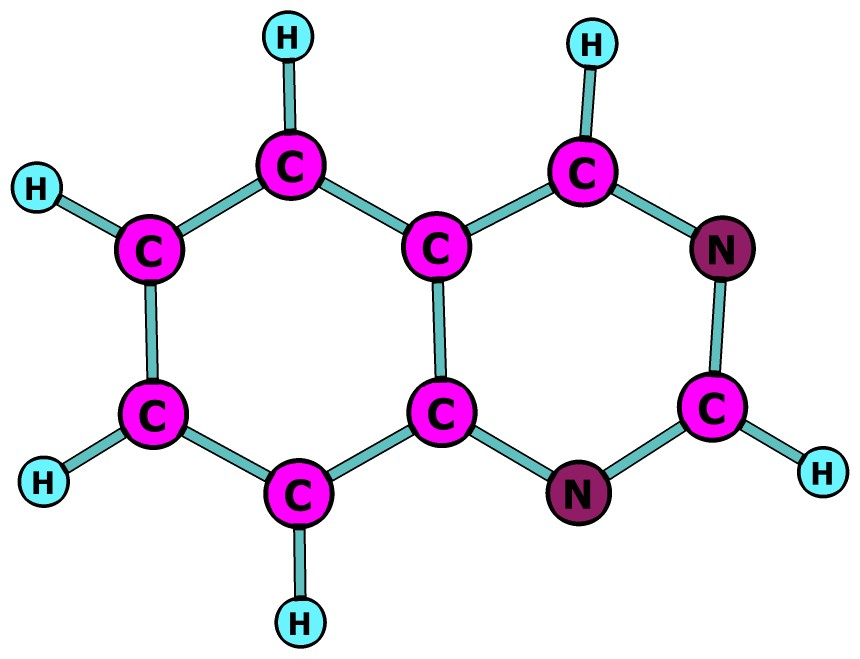
\includegraphics[scale=0.4]{fig/1.jpg}
\caption{Молекулы хиназолина}
\end{figure}